% !TEX encoding = UTF-8
% !TEX TS-program = pdflatex
% !TEX root = ../tesi.tex
% !TEX spellcheck = it-IT

%**************************************************************
\chapter{Valutazioni retrospettive}
\label{cap:valutazioni-retrospettive}
\textbf{TODO: Aggiungere sintesi al capitolo}\\
%**************************************************************

%\intro{Aggiungere abstract}\\

\section{Obiettivi raggiunti}

\section{Problematiche riscontrate}

\section{Bilancio formativo}
\subsection{Il prima}
\subsection{Il dopo}

\section{Valutazione critica del Corso di Laurea}



\newpage

%\begin{figure}[!h] 
%    \centering 
%    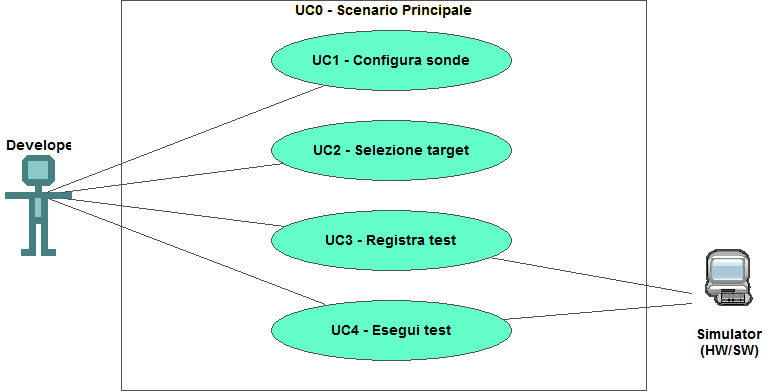
\includegraphics[width=0.9\columnwidth]{usecase/scenario-principale} 
%    \caption{Use Case - UC0: Scenario principale}
%\end{figure}

%\begin{usecase}{0}{Scenario principale}
%\usecaseactors{Sviluppatore applicativi}
%\usecasepre{Lo sviluppatore è entrato nel plug-in di simulazione all'interno dell'IDE}
%\usecasedesc{La finestra di simulazione mette a disposizione i comandi per configurare, registrare o eseguire un test}
%\usecasepost{Il sistema è pronto per permettere una nuova interazione}
%\label{uc:scenario-principale}
%\end{usecase}


%\begin{enumerate}
%	\item[R =] requisito
%    \item[F =] funzionale
%    \item[Q =] qualitativo
%    \item[V =] di vincolo
%    \item[N =] obbligatorio (necessario)
%    \item[D =] desiderabile
%    \item[Z =] opzionale
%\end{enumerate}
%Nelle tabelle \ref{tab:requisiti-funzionali}, \ref{tab:requisiti-qualitativi} e \ref{tab:requisiti-vincolo} sono riassunti i requisiti e il loro tracciamento con gli use case delineati in fase di analisi.



%\begin{table}%
%\caption{Tabella del tracciamento dei requisti funzionali}
%\label{tab:requisiti-funzionali}
%\begin{tabularx}{\textwidth}{lXl}
%\hline\hline
%\textbf{Requisito} & \textbf{Descrizione} & \textbf{Use Case}\\
%\hline
%RFN-1     & L'interfaccia permette di configurare il tipo di sonde del test & UC1 \\
%\hline
%\end{tabularx}
%\end{table}%

%\begin{table}%
%\caption{Tabella del tracciamento dei requisiti qualitativi}
%\label{tab:requisiti-qualitativi}
%\begin{tabularx}{\textwidth}{lXl}
%\hline\hline
%\textbf{Requisito} & \textbf{Descrizione} & \textbf{Use Case}\\
%\hline
%RQD-1    & Le prestazioni del simulatore hardware deve garantire la giusta esecuzione dei test e non la generazione di falsi negativi & - \\
%\hline
%\end{tabularx}
%\end{table}%

%\begin{table}%
%\caption{Tabella del tracciamento dei requisiti di vincolo}
%\label{tab:requisiti-vincolo}
%\begin{tabularx}{\textwidth}{lXl}
%\hline\hline
%\textbf{Requisito} & \textbf{Descrizione} & \textbf{Use Case}\\
%\hline
%RVO-1    & La libreria per l'esecuzione dei test automatici deve essere riutilizzabile & - \\
%\hline
%\end{tabularx}
%\end{table}%